% ============================================================
%  NotebookBuildAudit-Complete
%  Merged document: NotebookBuildAudit.tex (theoretical framework)
%  + InitialProposalDev.tex (commercial proposal)
%  Organized under a unified structure:
%    1. Codificar Experiencia Humana → Human-in-the-Loop Validation
%    2. Architecture (Conceptual → Logical → Physical)
%    3. Computational Costs
%    4. Energetic Costs — Proposal for a Third Pillar
%
%  Compile with: pdflatex (twice) or latexmk -pdf
% ============================================================
\documentclass[11pt, a4paper]{article}

% ── Packages ────────────────────────────────────────────────
\usepackage[T1]{fontenc}
\usepackage[utf8]{inputenc}
\usepackage[margin=2.4cm, top=2.8cm, bottom=2.8cm]{geometry}
\usepackage[expansion=false]{microtype}
\usepackage{parskip}
\usepackage{amsmath}
\usepackage{booktabs}
\usepackage{array}
\usepackage{tabularx}
\usepackage{adjustbox}
\usepackage{hyperref}
\usepackage{xcolor}
\usepackage{enumitem}
\usepackage{float}
\usepackage{caption}
\usepackage{listings}

% ── TikZ ────────────────────────────────────────────────────
\usepackage{tikz}
\usetikzlibrary{
  shapes.geometric,
  arrows.meta,
  positioning,
  fit,
  backgrounds,
  calc
}

% ── Forest (tree diagrams) ──────────────────────────────────
\usepackage{forest}
\forestset{
  mono tree/.style={
    for tree={
      calign=center,
      l sep=8mm,
      s sep=6mm,
      inner sep=4pt,
      draw,
      rounded corners=3pt,
      line width=0.4pt,
      font=\small\sffamily,
      text width=2.4cm,
      align=center,
    }
  }
}

% ── Colour definitions ──────────────────────────────────────
\definecolor{grayFill}{HTML}{D3D1C7}
\definecolor{grayStroke}{HTML}{888780}
\definecolor{grayTxt}{HTML}{2C2C2A}
\definecolor{axisFill}{HTML}{F1EFE8}
\definecolor{axisTxt}{HTML}{5F5E5A}
\definecolor{tealFill}{HTML}{9FE1CB}
\definecolor{tealStroke}{HTML}{0F6E56}
\definecolor{tealTxt}{HTML}{04342C}
\definecolor{purpleFill}{HTML}{CECBF6}
\definecolor{purpleStroke}{HTML}{534AB7}
\definecolor{purpleTxt}{HTML}{26215C}
\definecolor{coralFill}{HTML}{F5C4B3}
\definecolor{coralStroke}{HTML}{993C1D}
\definecolor{coralTxt}{HTML}{4A1B0C}
\definecolor{dashColor}{HTML}{B4B2A9}

\definecolor{clrBlue}{HTML}{2563EB}
\definecolor{clrGray}{HTML}{6B7280}
\definecolor{clrGreen}{HTML}{059669}
\definecolor{clrAmber}{HTML}{D97706}

% ── List style ──────────────────────────────────────────────
\setlist[description]{font=\normalfont\itshape}
\setlist[enumerate]{font=\normalfont}

% ── Column types ───────────────────────────────────────────
\newcolumntype{Y}{>{\raggedright\arraybackslash}X}
\newcolumntype{R}{>{\raggedleft\arraybackslash}p{3.5cm}}
\newcolumntype{L}{>{\raggedright\arraybackslash}p{3cm}}

% ── Hyperref ────────────────────────────────────────────────
\hypersetup{
  colorlinks=true,
  linkcolor=clrBlue,
  urlcolor=clrBlue,
  citecolor=clrBlue
}

% ── TikZ node styles ───────────────────────────────────────
\tikzset{
  base/.style={
    rectangle, rounded corners=5pt,
    text width=4.0cm, align=center,
    minimum height=1.1cm,
    inner sep=6pt,
    draw, line width=0.4pt,
    font=\small
  },
  gray node/.style={base,
    fill=grayFill, draw=grayStroke, text=grayTxt},
  axis node/.style={base,
    fill=axisFill, draw=dashColor,
    text=axisTxt, dashed,
    text width=12.8cm, minimum height=0.9cm},
  teal node/.style={base,
    fill=tealFill, draw=tealStroke, text=tealTxt},
  purple node/.style={base,
    fill=purpleFill, draw=purpleStroke, text=purpleTxt},
  coral node/.style={base,
    fill=coralFill, draw=coralStroke, text=coralTxt},
}

% ── Listings style for prompts ─────────────────────────────
\lstdefinestyle{promptStyle}{
  basicstyle=\small\sffamily,
  breaklines=true,
  breakatwhitespace=true,
  frame=single,
  framesep=4pt,
  rulecolor=\color{grayStroke},
  backgroundcolor=\color{axisFill},
  xleftmargin=8pt,
  xrightmargin=8pt,
  aboveskip=8pt,
  belowskip=8pt
}

% ============================================================
\begin{document}

% ============================================================
%  Title Page
% ============================================================
\begin{titlepage}
  \centering
  \vspace*{3cm}

  {\Huge\bfseries Notebook Build Audit}\\[0.4cm]
  {\Huge\bfseries \& Execution System}\\[1cm]
  {\Large Unified Framework Specification}\\[0.5cm]
  {\large Construction, Audit, and Resource Analysis}\\[3cm]

  \vfill

  {\large\textit{``Codificar experiencia humana, validar con supervisión
  sistemática.''}}\\[0.3cm]
  {\footnotesize\color{clrGray} — Encoding human expertise, validating through
  systematic oversight}\\[2cm]

  {\footnotesize\color{clrGray} Compiled from: NotebookBuildAudit.tex \&
  InitialProposalDev.tex}\\[0.2cm]
  {\footnotesize\color{clrGray} \today}
  \vspace*{2cm}
\end{titlepage}

% ============================================================
%  Table of Contents
% ============================================================
\newpage
\tableofcontents
\newpage

% ============================================================
%  Part I — Codificar Experiencia Humana
% ============================================================
\part{Codificar Experiencia Humana}

The fundamental thesis of this work is that rigorous notebook engineering
requires \textit{encoding human expertise} into repeatable, verifiable
structures — and then \textit{validating} those structures through a
systematic, human-in-the-loop audit protocol. This part presents the two
complementary frameworks that realise this vision.

% ── Section 1: The Challenge ────────────────────────────────
\section{The Challenge}

Computational notebooks (\texttt{.ipynb}) have become the dominant medium for
data science and machine learning workflows. However, they introduce systemic
risks that compromise reproducibility, correctness, and auditability at every
stage of the lifecycle:

\begin{itemize}
  \item \textbf{Untrusted notebook execution} — notebooks often originate from
    external collaborators, open-source repositories, or AI-assisted code
    generation without any deterministic guarantee that they run safely or
    correctly.

  \item \textbf{Lack of deterministic builds} — ad hoc environment pinning,
    missing dependency declarations, and absent seed controls cause notebooks
    to produce different results across machines or sessions, undermining
    scientific validity.

  \item \textbf{No structured audit protocol} — teams lack a systematic,
    multi-pass methodology for reviewing notebooks before production
    deployment, publication, or merge. Existing code review practices are
    insufficient for the unique failure modes of notebook-based ML pipelines:
    data leakage through preprocessing ordering, cross-validation
    contamination, inseparable training/inference logic.
\end{itemize}

The \textbf{Notebook Build Audit \& Execution System} addresses these gaps
through two tightly coupled frameworks: a forward-looking \textit{Construction
Framework} that guides notebook authors in producing well-structured
artifacts, and a backward-looking \textit{Audit Framework} that systematically
diagnoses weaknesses in existing notebooks.

% ── Section 2: Construction Framework ──────────────────────
\section{Notebook Construction Framework}
\label{sec:construction}

The Construction Framework is a \textit{forward-looking prescription}: it
guides the notebook author in producing a well-structured, reproducible, and
maintainable artifact from the ground up. It is organized into three
sequential phases.

% ── Diagram: Construction Strategy Tree ────────────────────
\begin{figure}[ht]
  \centering
  \resizebox{\textwidth}{!}{%
    \begin{forest}
      mono tree,
      [Notebook Construction\\Strategy
        [Modular\\Section Design]
        [{Reproducibility Standards\\(seeds, environments)}]
        [Narrative Documentation\\Guidelines]
        [Output Artifact\\Management]
      ]
    \end{forest}
  }
  \caption{High-level pillars of the Notebook Construction Framework.}
  \label{fig:construction-tree}
\end{figure}

\subsection*{Phase 1 — Scaffold}

Establish the structural and reproducibility foundation before writing any
logic:

\begin{itemize}
  \item Define the notebook's \textbf{single responsibility} — one notebook
    should correspond to one coherent workflow or experiment.

  \item Create standard section headers as markdown cells, following this
    canonical order:
  \begin{enumerate}
    \item Environment \& Dependencies
    \item Configuration \& Global Parameters
    \item Data Ingestion
    \item Preprocessing \& Feature Engineering
    \item Model Definition \& Training
    \item Evaluation \& Metrics
    \item Artifact Export (models, plots, reports)
    \item Conclusions \& Next Steps
  \end{enumerate}

  \item Pin the execution environment upfront via \texttt{requirements.txt},
    \texttt{conda.yaml}, or \texttt{pyproject.toml}.

  \item Set global reproducibility controls: random seeds, deterministic
    flags, and device configuration.
\end{itemize}

\subsection*{Phase 2 — Write}

Author each section incrementally, following these discipline rules:

\begin{itemize}
  \item Work through \textbf{one section at a time} (Divide and Conquer
    principle).

  \item Accompany every code cell with a markdown explanation of intent and
    expected output.

  \item Avoid burying logic inside loops or helper calls without commentary.

  \item Prefer \textbf{explicit variable passing} over hidden or global state
    to maintain cell independence.

  \item Summarise repetitive code patterns with a general description and
    highlight meaningful variations; three or more similar blocks should be
    treated as a refactoring candidate.

  \item Route all persisted outputs (models, plots, reports) through a single,
    versioned export convention defined at the start of the section — never
    write artifacts ad hoc from arbitrary cells.
\end{itemize}

\subsection*{Phase 3 — Validate During Writing}

Continuously verify correctness as each section is completed:

\begin{itemize}
  \item Restart the kernel and run all cells after completing each section.

  \item Confirm \textbf{cell idempotency}: every cell should produce the same
    result when re-executed independently.

  \item Verify that outputs match expectations before proceeding to the next
    section.

  \item Ensure cell execution order is strictly linear and free of hidden
    dependencies.

  \item Confirm that exported artifacts land in the designated output location
    with the expected naming and versioning convention before moving to the
    next section.
\end{itemize}

The Construction Framework encodes human expertise about \textit{how to build
rigorous notebooks} into a repeatable process. The expertise — section
discipline, reproducibility hygiene, incremental validation — is the
``codified experience'' that the author brings to each new notebook.

% ── Section 3: LLM-as-a-Judge Paradigm ─────────────────────
\section{LLM-as-a-Judge as the Evaluation Paradigm}
\label{sec:laj}

The proposed notebook auditing framework follows the emerging
\textbf{LLM-as-a-Judge (LAJ)} paradigm~\cite{zheng2023judging}, in which a
powerful language model evaluates the outputs of another model (or of itself
under controlled prompting) instead of relying solely on human reviewers.
This approach is particularly suitable for notebook audits because many
evaluation criteria --- such as code clarity, logical coherence,
documentation quality, or methodological soundness --- cannot be measured
using deterministic metrics alone.

Unlike traditional automatic evaluation metrics (e.g., BLEU or ROUGE), which
require reference outputs and perform poorly on open-ended reasoning tasks,
an LLM judge can evaluate responses using qualitative criteria similar to
those employed by expert reviewers. Recent work has shown that sufficiently
capable language models achieve agreement with human evaluators comparable to
inter-human agreement when judging open-ended responses~\cite{zheng2023judging}.

\subsection{Motivation}

Notebook auditing combines objective and subjective evaluation tasks.

\textbf{Objective tasks} include:
\begin{itemize}
  \item dependency validation,
  \item execution reproducibility,
  \item train/test split verification,
  \item artifact existence,
  \item environment completeness.
\end{itemize}
These can often be evaluated deterministically through programmatic checks.

Conversely, \textbf{subjective tasks} include:
\begin{itemize}
  \item quality of documentation,
  \item conceptual coherence,
  \item methodological soundness,
  \item explanation quality,
  \item maintainability,
  \item deployment readiness.
\end{itemize}
These require semantic reasoning and therefore benefit from an LLM acting as
an evaluator.

The proposed framework intentionally separates these two categories rather
than attempting to solve both with a single mechanism.

\subsection{Deterministic Evaluation vs.\ LLM Judging}

The audit framework adopts a layered evaluation strategy.

\subsubsection*{Layer 1 — Deterministic Verification}

Whenever correctness can be established objectively, deterministic evaluation
is preferred. Examples include:
\begin{itemize}
  \item successful notebook execution,
  \item dependency resolution,
  \item version pinning,
  \item artifact generation,
  \item file existence,
  \item reproducibility checks.
\end{itemize}
These evaluations are binary and reproducible.

\subsubsection*{Layer 2 — LLM-as-a-Judge}

Only after deterministic checks have been completed does the framework invoke
an LLM judge to assess properties requiring semantic interpretation. Examples
include:
\begin{itemize}
  \item structural organisation,
  \item readability,
  \item methodological consistency,
  \item code explanation quality,
  \item deployment recommendations.
\end{itemize}

This mirrors the evaluation philosophy adopted by recent agent benchmarks,
where objective verification forms the first layer of validation while
model-based evaluation is reserved for inherently subjective tasks.

\subsubsection*{Budget-Aware Allocation (ROBIN-HOOD)}

A critical practical consideration arises because LLM judgments are
stochastic --- querying the same pair multiple times yields different scores
due to sampling randomness. Score variance is highly heterogeneous: a factual
check like ``dependency resolution'' may have variance near zero, while a
subjective assessment like ``methodological soundness'' can vary
significantly. Given a fixed query budget $B$ across $K$ evaluation pairs,
optimal allocation is non-trivial~\cite{saha2026robinhood}.

Recent work formalises this as a multi-armed bandit problem: each pair is an
arm with unknown mean $s_i$ and variance $\sigma_i^2$, and the goal is to
minimise worst-case estimation error $\max_i |s_i - \hat{s}_i|$ under budget
$B$. The \textbf{ROBIN-HOOD} algorithm~\cite{saha2026robinhood} dynamically
allocates queries based on estimated score variances using upper confidence
bounds, concentrating resources where uncertainty is highest. It achieves a
worst-case error of $\tilde{O}\big(\sqrt{\sum_i \sigma_i^2 / B}\big)$ with
near-optimal allocation, and experiments on \texttt{HelpSteer2} show it
matches uniform allocation accuracy at \textbf{half the budget}.

This is directly relevant to the notebook audit framework: the six-pass
protocol contains both low-variance passes (Structural Overview,
Reproducibility Check) and high-variance passes (ML Correctness Audit,
Deployment Readiness). A production system should therefore weight its LLM
query budget toward passes where the evaluation is most uncertain, rather
than querying each pass uniformly.

\subsection{Prompt Engineering as Judge Design}

An LLM judge is only as reliable as its evaluation
protocol~\cite{liu2023geval}.

Following the G-Eval methodology, the prompts presented in this work do not
ask the model to provide a single holistic score. Instead, each prompt
decomposes notebook evaluation into explicit review criteria.

Rather than asking

\begin{quote}
  ``Is this notebook good?''
\end{quote}

the evaluator is instructed to inspect predefined dimensions such as:
\begin{itemize}
  \item reproducibility,
  \item data integrity,
  \item methodological correctness,
  \item implementation quality,
  \item deployment readiness.
\end{itemize}

The resulting structured reports resemble formal peer-review checklists
instead of free-form opinions, improving consistency across repeated
evaluations.

This principle directly motivates the progressive prompt hierarchy introduced
in Section~\ref{sec:prompt-crafting}, where increasingly constrained prompts
guide the model from coarse inspection toward structured multi-pass auditing.

\subsection{Known Limitations}

Although LLM judges exhibit strong agreement with human evaluators, they
remain susceptible to systematic biases~\cite{wang2024bias,zhang2024evalbias}:

\begin{itemize}
  \item \textbf{Position bias} --- preference for the first candidate
    presented.
  \item \textbf{Verbosity bias} --- longer responses often receive higher
    scores despite similar quality.
  \item \textbf{Self-enhancement bias} --- models tend to rate their own
    generations more favourably than those produced by competing models.
  \item \textbf{Reasoning limitations} --- evaluation quality decreases when
    the judge must solve difficult mathematical or logical problems before
    assessing correctness.
\end{itemize}

These limitations motivate the design choices adopted throughout the audit
framework:
\begin{itemize}
  \item decomposition into multiple audit passes,
  \item explicit evaluation criteria,
  \item preference for deterministic verification whenever possible,
  \item avoidance of single holistic quality scores.
\end{itemize}

Rather than treating the LLM as an oracle, the framework views it as a
structured reviewer operating within clearly defined evaluation boundaries.

\subsection*{The Generation--Evaluation Dissociation}

A deeper structural limitation, recently formalised by the \textit{Metanym
Game}~\cite{nordfors2026metanym}, is that \textbf{generating and evaluating
are dissociated skills}. In a peer-community benchmark where LLMs both create
content and rate each other's creations, singular value decomposition of the
ratings matrix reveals that:

\begin{itemize}
  \item The strongest generators are \textbf{middling judges} --- producing
    high-quality content does not imply the ability to evaluate it reliably.

  \item The sharpest judges are \textbf{mid-pack generators} --- evaluation
    skill is scarcer and partially independent of generative capability.

  \item Factual rating competence correlates with GPQA Diamond at $r = 0.92$,
    validating that the spectral decomposition recovers genuine evaluation
    ability.
\end{itemize}

This finding has direct implications for notebook auditing: using the same
LLM model to generate audit reports (Passes 1--6) and to evaluate their own
correctness may conflate two distinct capabilities. A more robust design,
following the ``jury'' proposal~\cite{verga2024juries}, would employ a
\textbf{panel of diverse models} --- some optimised for structured reasoning
(Passes 3--4), others for stylistic judgment (Passes 5--6) --- and aggregate
their assessments to mitigate individual model biases.

\subsection{Position within This Work}

The notebook auditing framework proposed in this document should therefore be
interpreted as a specialised instance of the LLM-as-a-Judge paradigm.

Its primary contribution is not a new evaluation model, but a structured
auditing protocol that combines:
\begin{enumerate}
  \item deterministic verification wherever objective correctness exists;
  \item prompt-engineered LLM judging for semantic evaluation;
  \item incremental multi-pass analysis that progressively refines the
    assessment while reducing cognitive overload for both the evaluator and
    the reader.
\end{enumerate}

This hybrid strategy combines the reproducibility of automated software
testing with the flexibility of modern language-model evaluation, providing a
practical methodology for AI-assisted review of computational notebooks.

\subsection*{Extensions Informed by Recent Advances}

Two lines of recent work directly extend the framework's practical reach:

\begin{description}
  \item[Budget-aware query allocation.] The ROBIN-HOOD
    algorithm~\cite{saha2026robinhood} addresses a critical operational
    question: given a fixed LLM query budget, how should it be distributed
    across the six passes to minimise worst-case estimation error? Because
    pass variance differs (low for Reproducibility Check, high for ML
    Correctness Audit), a variance-adaptive allocation significantly
    outperforms uniform querying. This is the natural next step for a
    production deployment.

  \item[Panel-based evaluation (jury).] The Metanym
    Game~\cite{nordfors2026metanym} demonstrates that generating and
    evaluating are dissociated skills --- the best generators are not the
    best judges. Combined with the jury proposal~\cite{verga2024juries}, this
    motivates replacing a single LLM judge with a \textbf{council of diverse
    models}, each specialising in passes aligned with its strengths (e.g., a
    smaller model for structural checks, a larger one for ML correctness).
    The architecture's existing \texttt{LLMProvider} strategy pattern already
    supports this extension without structural changes.
\end{description}

% ── Section 4: Prompt Crafting — Encoding Expert Knowledge ─
\section{Prompt Crafting --- Encoding Expert Knowledge}
\label{sec:prompt-crafting}

To operationalise the Construction and Audit frameworks through an LLM, human
expertise must be encoded into structured prompts that guide the model's
reasoning. This section presents a three-level prompt engineering framework
that maps cleanly onto the six-pass audit protocol.

\subsection*{The Three-Level Structure}

\begin{enumerate}
  \item \textbf{Level 1 — Conceptual} (Passes 1--2): Structural Overview +
    Reproducibility Check. Establishes whether the notebook is coherent and
    re-runnable at all, before any deep inspection is worth doing.

  \item \textbf{Level 2 — Methodological} (Passes 3--4): Data Integrity
    Review + ML Correctness Audit. Addresses whether the pipeline and
    modelling logic are scientifically sound — the ``does this work
    correctly?'' layer.

  \item \textbf{Level 3 — Implementation} (Passes 5--6): Code Quality Review +
    Deployment Readiness. Addresses \textit{how} the working logic is written
    and packaged — the most granular, code-level layer.
\end{enumerate}

\subsection*{Prompt Iterations (Lap Progression)}

The prompt templates themselves evolve through successive refinements:

\begin{description}
  \item[Lap 1 — Coarse Evaluation:] A broad, unstructured task statement that
    asks the LLM to analyse the notebook holistically. It requests a phase 1
    documentation (purpose, code block descriptions, pseudocode for complex
    functions) and a phase 2 critical audit (cross-block consistency,
    redundancy, contradictory logic, error handling). Yields an initial gate
    decision.

  \item[Lap 2 — Refined Evaluation:] Introduces structural rules for block
    numbering (visual order, not execution order), consolidation of imports
    into a single ``Environment Setup'' block, filtering of markdown and error
    cells, and explicit output format requirements. Adds a five-point
    extraction template: Logic Flow, Data Transformations, Model/Algorithm
    Operations, Key Variables/Parameters, Side Effects.

  \item[Lap 3 — Structured Evaluation:] Formalises the three-level hierarchy
    (Conceptual, Methodological, Implementation) as a deterministic mapping
    onto the six-pass framework. Each level has its own deliverable
    requirements, gate decisions, and scoring rubric.
\end{description}

\subsection*{Level 1 — Conceptual Purpose (Detail)}

This level determines whether the notebook is coherent and reliably
re-executable before investing time in deeper review.

\textbf{Procedure:}
\begin{enumerate}
  \item \textit{Scope the audit} — Record user-specified focus areas or
    exclusions.
  \item \textit{Map the structure} — Assess section headers, confirm single
    coherent purpose, verify linear execution order.
  \item \textit{Scan for immediate red flags} — Missing outputs, broken
    imports, orphaned cells.
  \item \textit{Check reproducibility inputs} — Dependency pinning, global
    seed configuration.
  \item \textit{Check reproducibility risks} — Hardcoded paths, credentials,
    environment-specific assumptions.
\end{enumerate}

\textbf{Deliverables:} Section map, preliminary red flags list, recorded
focus-area scope, reproducibility risk score (Low / Moderate / High).

\textbf{Gate decision:} If the notebook fails end-to-end execution or lacks a
coherent single purpose, decide whether to proceed to Level 2 or flag Level 1
as blocking.

\subsection*{Level 2 — Methodological Purpose (Detail)}

This level evaluates the scientific soundness of the data pipeline and ML
methodology.

\textbf{Procedure:}
\begin{enumerate}
  \item \textit{Audit the data pipeline} — Train/test split ordering,
    data leakage detection, missing-data consistency, type/shape validation at
    ingestion.
  \item \textit{Audit ML correctness} — Metric appropriateness, cross-
    validation integrity, hyperparameter tuning boundaries, baseline
    comparison.
  \item \textit{Cross-check across pipeline stages} — Verify that
    transformations applied during preprocessing are correctly reflected in
    downstream modelling and evaluation.
\end{enumerate}

\textbf{Deliverables:} Data pipeline integrity report, ML correctness
checklist.

\textbf{Gate decision:} If methodological flaws are found (leakage, invalid
cross-validation, metric misuse), decide whether to halt or proceed to Level
3 with flagged caveats.

\subsection*{Level 3 — Implementation Purpose (Detail)}

This level assesses code maintainability and production suitability.

\textbf{Procedure:}
\begin{enumerate}
  \item \textit{Code quality review} — Identify repetitive blocks (three-block
    threshold), dead code, naming quality, output hygiene.
  \item \textit{Deployment readiness check} — Versioned artifact export,
    inference/training separability, resource documentation, environment
    completeness, data privacy.
\end{enumerate}

\textbf{Deliverables:} Code quality and smell report, deployment readiness
score (Low / Moderate / High).

\subsection*{Weighted Evaluation Dimensions}

For external audits (e.g., markdown exports), a weighted multi-dimensional
scoring system is used:

\begin{itemize}
  \item \textbf{Reproducibility \& Self-Containment (40\%)} — Highest
    priority. Dependency declarations, output expectations, placeholders.
  \item \textbf{Narrative \& Structure (35\%)} — Section transitions, heading
    hierarchy, audience identification, reading flow.
  \item \textbf{Purpose \& Depth (25\%)} — Explicit primary purpose, learning
    path (tutorials), hypothesis--method--results separation (experiments),
    interpretable outputs.
\end{itemize}

This weighted system ensures that critical reproducibility and structural
flaws receive proportionate attention before stylistic or depth-based
concerns.

% ── Section 5: Audit Framework — Human-in-the-Loop Validation
\section{Audit Framework — Human-in-the-Loop Validation}
\label{sec:audit}

The Audit Framework is a \textit{backward-looking diagnostic}: it guides a
reviewer, collaborator, or AI assistant in systematically assessing the
quality, correctness, and risk profile of an existing notebook.

\subsection*{Guiding Tactics}

Before executing the passes, the reviewer employs these tactics:

\begin{itemize}
  \item Divide the notebook into logical modules, prioritising critical ML
    pipeline blocks over repetitive exploration cells.
  \item Use hierarchical descriptions: high-level summaries first, drill-downs
    later.
  \item Summarise repetitive code patterns rather than analysing each
    individually.
  \item When a human collaborator specifies focus areas in advance, scope the
    six-pass protocol to those areas rather than executing all passes
    uniformly.
\end{itemize}

\subsection*{The Six-Pass Audit Protocol}

Where a pass deliverable is a score, the reviewer rates on a three-level scale
— \textit{Low Risk}, \textit{Moderate Risk}, \textit{High Risk} — based on
the number and severity of unresolved items identified within that pass.

% ── Diagram: Audit Strategy Tree ───────────────────────────
\begin{figure}[ht]
  \centering
  \resizebox{\textwidth}{!}{%
    \begin{forest}
      mono tree,
      [Notebook Audit\\Strategy
        [{Multi-Pass Incremental\\Analysis}]
        [Hierarchical\\Review Depth]
        [Pattern Summarization\\with Thresholds]
        [{User-Guided Focus Areas\\(AI-assisted context)}]
      ]
    \end{forest}
  }
  \caption{High-level pillars of the Notebook Audit Framework.}
  \label{fig:audit-tree}
\end{figure}

\begin{description}

  \item[Pass 1 — Structural Overview:]
  Establish a high-level map of the notebook before examining any logic:
  \begin{itemize}
    \item Record any user-specified focus areas or exclusions.
    \item Assess clear, navigable section headers and single coherent purpose.
    \item Verify linear, safe cell execution order.
    \item Identify immediately visible red flags (missing outputs, broken
      imports, orphaned cells).
  \end{itemize}
  \textit{Deliverable:} Section map, preliminary red flags list, recorded
  focus-area scope.

  \item[Pass 2 — Reproducibility Check:]
  Assess whether the notebook can be reliably re-executed:
  \begin{itemize}
    \item Verify dependency pinning (\texttt{requirements.txt},
      \texttt{conda.yaml}).
    \item Confirm global, consistent random seed configuration.
    \item Flag hardcoded file paths, credentials, environment assumptions.
    \item Determine end-to-end runnability on a fresh kernel.
  \end{itemize}
  \textit{Deliverable:} Reproducibility risk score (Low / Moderate / High).

  \item[Pass 3 — Data Integrity Review:]
  Examine the data pipeline for correctness and leakage risks:
  \begin{itemize}
    \item Confirm train/test split is performed \textbf{before} any
      preprocessing.
    \item Identify data leakage (e.g., scaling fitted on full dataset).
    \item Verify consistent missing-data handling across splits.
    \item Check data type, shape, and distribution validation at ingestion.
  \end{itemize}
  \textit{Deliverable:} Data pipeline integrity report.

  \item[Pass 4 — ML Correctness Audit:]
  Evaluate the soundness of the machine learning methodology:
  \begin{itemize}
    \item Confirm metric appropriateness for task and class distribution.
    \item Verify correct cross-validation application without leakage.
    \item Ensure hyperparameter tuning uses validation data only.
    \item Check performance contextualisation against a meaningful baseline.
  \end{itemize}
  \textit{Deliverable:} ML correctness checklist.

  \item[Pass 5 — Code Quality Review:]
  Assess maintainability and clarity of the code:
  \begin{itemize}
    \item Flag repetitive blocks exceeding the three-block threshold.
    \item Identify dead code, unused imports, redundant assignments.
    \item Assess meaningful and consistent variable/function naming.
    \item Check for bloated cell outputs.
  \end{itemize}
  \textit{Deliverable:} Code quality and smell report.

  \item[Pass 6 — Deployment Readiness:]
  Determine production or publication suitability:
  \begin{itemize}
    \item Verify versioned model artifact export.
    \item Confirm separable inference and training logic.
    \item Check documented compute and memory constraints.
    \item Ensure complete, up-to-date environment export.
    \item Flag data privacy or PII handling concerns.
  \end{itemize}
  \textit{Deliverable:} Deployment readiness score (Low / Moderate / High).

\end{description}

\subsection*{Applying the Two Frameworks}
\label{sec:applying}

The appropriate framework depends on the context of engagement with the
notebook:

\begin{description}
  \item[Use the Construction Framework when:] starting a new notebook or
    experiment; restructuring a disorganised notebook from scratch; or creating
    a reusable notebook template.

  \item[Use the Audit Framework when:] reviewing a collaborator's notebook;
    preparing for production deployment or academic publication; conducting a
    pre-merge or pre-deployment review.

  \item[Use Both Frameworks iteratively when:] authoring and self-reviewing
    during active development; collaborating or pair-programming in real time;
    or refactoring an existing notebook while preserving its structure.
\end{description}

The two frameworks form a feedback loop:

\begin{quote}
  Construction Phase $\rightarrow$ produces notebook artifact $\rightarrow$
  Audit Phase $\rightarrow$ diagnoses weaknesses $\rightarrow$
  recommendations feed back into revised Construction $\rightarrow$ \ldots
\end{quote}

This closure applies to notebooks that begin in the Building Phase. For
notebooks entering via the audit-only path, the loop remains open unless the
notebook is subsequently revised.

% ============================================================
%  Part II — Architecture
% ============================================================
\part{Architecture}

This part presents the system architecture at three levels of abstraction:
conceptual (the mental model), logical (the component model), and physical
(the deployment model).

% ── Section 6: Conceptual Architecture ─────────────────────
\section{Conceptual Architecture}
\label{sec:conceptual-arch}

The conceptual architecture is defined by the relationship between the two
frameworks and the three-level audit model that governs LLM-driven analysis.

\subsection*{Core Concepts}

\begin{itemize}
  \item \textbf{Notebook Lifecycle} — A notebook exists in one of two states:
    under construction (authoring) or under audit (review). The feedback loop
    connects both states.

  \item \textbf{Three-Level Audit Model} — The six-pass protocol is grouped
    into three levels (Conceptual, Methodological, Implementation) that
    correspond to increasing depth of analysis. Gate decisions between levels
    allow early termination when blocking issues are found.

  \item \textbf{Human-in-the-Loop} — The system is diagnostic, not
    prescriptive. Every gate decision and pass deliverable is presented to a
    human reviewer who makes the final call. The LLM provides structured
    evidence; the human provides judgment.

  \item \textbf{Provider Agnosticism} — The LLM orchestration layer
    abstracts over local (Ollama, \texttt{llama.cpp}) and cloud (OpenAI)
    providers through a strategy pattern, allowing the same audit logic to
    run in air-gapped or connected environments.
\end{itemize}

\subsection*{Framework Feedback Loop}

\begin{figure}[ht]
  \centering
  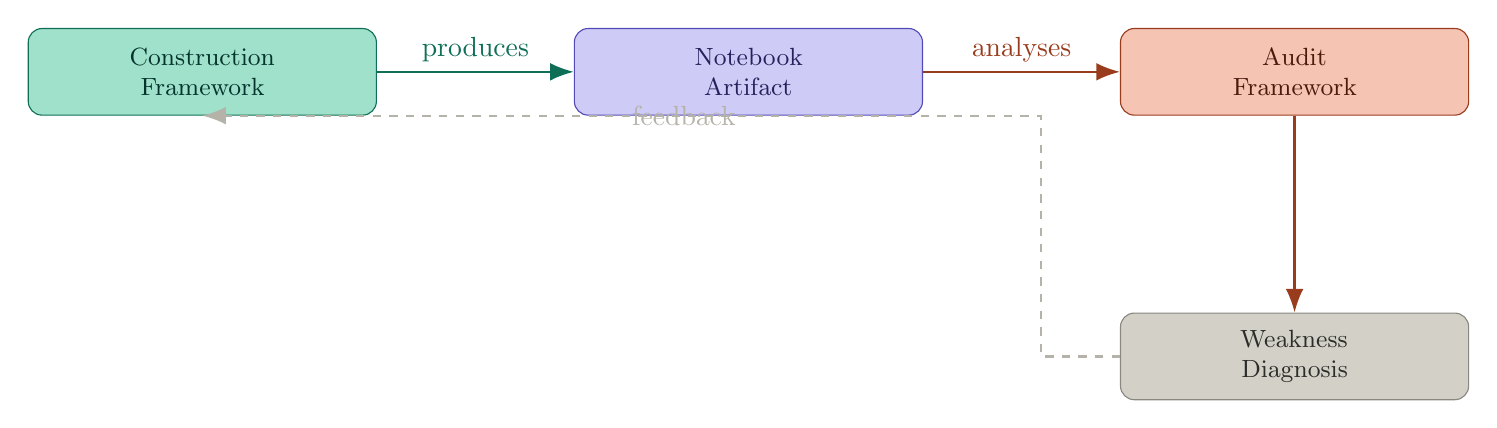
\begin{tikzpicture}[node distance=2.5cm, auto]
    % Nodes
    \node[teal node] (construction) {Construction\\Framework};
    \node[purple node, right=of construction] (artifact) {Notebook\\Artifact};
    \node[coral node, right=of artifact] (audit) {Audit\\Framework};
    \node[gray node, below=of audit] (findings) {Weakness\\Diagnosis};

    % Arrows
    \draw[-{Latex[length=3mm]}, tealStroke, thick]
      (construction) -- node[above] {produces} (artifact);
    \draw[-{Latex[length=3mm]}, coralStroke, thick]
      (artifact) -- node[above] {analyses} (audit);
    \draw[-{Latex[length=3mm]}, coralStroke, thick]
      (audit) -- (findings);
    \draw[-{Latex[length=3mm]}, dashColor, thick, dashed]
      (findings.west) -- ++(-1,0) |- (construction.south)
      node[pos=0.75, right] {feedback};
  \end{tikzpicture}
  \caption{Conceptual feedback loop between the Construction and Audit
           Frameworks.}
  \label{fig:lifecycle}
\end{figure}

% ── Section 6: Logical Architecture ─────────────────────────
\section{Logical Architecture}
\label{sec:logical-arch}

The logical architecture decomposes the system into its core components and
their responsibilities.

\subsection*{System Components}

\begin{figure}[ht]
  \centering
  \begin{verbatim}
[React + TypeScript Dashboard]  <-->  [FastAPI REST + SSE Gateway]
                                          |
                    +---------------------+---------------------+
                    |                     |                     |
              LLM Orchestrator     Audit State Machine   Jupyter Exec. Engine
              (Provider Strategy)  (Six-Pass Protocol)   (@jupyter-kit Sandbox)
                    |                     |                     |
              +-----+-----+           Audit Results DB      Docker Sandbox
              |           |           (PostgreSQL)          (per-notebook)
           Ollama      OpenAI
           (local)     (cloud)
  \end{verbatim}
  \caption{Logical component diagram of the Notebook Build Audit \& Execution
           System.}
  \label{fig:logical-arch}
\end{figure}

\subsection*{Component Responsibilities}

\begin{description}
  \item[React + TypeScript Dashboard:] Single-page application for audit
    session management, notebook upload, provider routing configuration,
    pass scope selection, and live audit progress visualisation. Communicates
    with the backend via REST and Server-Sent Events (SSE).

  \item[FastAPI REST + SSE Gateway:] Async-first Python backend exposing a
    REST API for audit session CRUD, notebook upload, and configuration. SSE
    endpoints stream per-pass audit deliverables in real time, enabling live
    progress without polling.

  \item[LLM Orchestrator (Provider Strategy):] Implements the
    \texttt{LLMProvider} abstract base class with concrete implementations for
    Ollama, \texttt{llama.cpp}, and OpenAI. The \texttt{LLMOrchestrator}
    service selects the appropriate provider at runtime based on audit
    configuration (privacy, latency, capability requirements). Prompt
    templates from the three-level framework are parameterised and injected
    per audit pass. The strategy pattern is designed to accept additional
    providers (Anthropic, OpenCode) post-launch without architectural changes.

  \item[Audit State Machine:] Each notebook audit is modelled as a state
    machine transitioning through \texttt{Scope $\rightarrow$ Pass1
    $\rightarrow$ Pass2 $\rightarrow$ \ldots $\rightarrow$ Pass6}. Gate
    decisions between Levels 1, 2, and 3 are configurable checkpoints — the
    system can halt at a blocking issue or continue to surface further
    findings.

  \item[Jupyter Execution Engine (@jupyter-kit):] Programmatic Jupyter kernel
    management, cell-level execution, output capture, and metadata inspection
    within a sandboxed Docker container.

  \item[PostgreSQL + SQLAlchemy 2.0 (async):] Relational storage for audit
    sessions, notebook metadata, audit results, and user configuration. Schema
    migrations managed via Alembic.
\end{description}

\subsection*{Key Architectural Decisions}

\begin{description}
  \item[Strategy Pattern for LLM Providers:] The \texttt{LLMProvider}
    abstract base class defines \texttt{generate(prompt, **kwargs)}. Concrete
    implementations handle provider-specific API formatting. Runtime provider
    selection is based on audit configuration — local providers for
    offline/privacy-sensitive audits, cloud providers for high-capability
    inference.

  \item[Audit State Machine:] State transitions with gate checkpoints. Each
    gate can be configured to halt on failure or continue with caveats,
    giving the human reviewer full control over audit depth.

  \item[Server-Sent Events for Real-Time Logs:] The FastAPI backend streams
    per-pass deliverables to the frontend via SSE, enabling live progress
    without polling overhead.
\end{description}

% ── Section 7: Physical Architecture ────────────────────────
\section{Physical Architecture}
\label{sec:physical-arch}

\subsection*{Deployment Topology}

The system is deployed via Docker Compose with the following services:

\begin{table}[H]
  \centering
  \caption{Physical deployment services.}
  \label{tab:deployment}
  \renewcommand{\arraystretch}{1.3}
  \begin{tabularx}{\textwidth}{l l Y}
    \toprule
    \textbf{Service} & \textbf{Image/Base} & \textbf{Role} \\
    \midrule
    Frontend & Node 20 + Vite build & Serves the React SPA \\
    Backend & Python 3.11+ / FastAPI & REST + SSE API \\
    Database & PostgreSQL 15 & Persistent storage \\
    Sandbox & Python 3.11+ (per-notebook) & Isolated \texttt{@jupyter-kit}
      execution \\
    LLM Local & Ollama / \texttt{llama.cpp} & On-device inference \\
    \bottomrule
  \end{tabularx}
\end{table}

\subsection*{Resource Isolation}

Each notebook audit spawns a short-lived Docker container with the notebook's
declared dependencies pre-installed. The container runs a headless Jupyter
kernel managed by \texttt{@jupyter-kit} and is destroyed after the audit
completes, providing full isolation between audit sessions.

\subsection*{Provider Deployment Options}

\begin{itemize}
  \item \textbf{Local (air-gapped):} Ollama or \texttt{llama.cpp} running on
    the same host or local network. Zero external API calls. Suitable for
    privacy-sensitive or regulated environments.

  \item \textbf{Cloud (high-capability):} OpenAI API (and potentially
    Anthropic, OpenCode) for maximum model capability. Requires internet
    connectivity and API key configuration.
\end{itemize}

% ============================================================
%  Part III — Computational Costs
% ============================================================
\part{Computational Costs}

This part analyses the computational resources required to operate the
system, covering infrastructure, LLM inference, and development investment.

% ── Section 8: Infrastructure Costs ─────────────────────────
\section{Infrastructure Costs}

\subsection*{Hardware Requirements}

The base deployment requires a server with the following minimum
specifications:

\begin{table}[H]
  \centering
  \caption{Minimum hardware requirements.}
  \label{tab:hardware}
  \renewcommand{\arraystretch}{1.3}
  \begin{tabularx}{\textwidth}{l Y}
    \toprule
    \textbf{Component} & \textbf{Specification} \\
    \midrule
    CPU & 8+ cores (x86\_64 or ARM64) \\
    RAM & 32\,GB minimum; 64\,GB recommended for local LLM inference \\
    GPU & Optional; NVIDIA with 8+ GB VRAM for local GPU-accelerated
      inference \\
    Storage & 100\,GB SSD (system + models + databases) \\
    Network & 100\,Mbps (cloud provider mode requires internet access) \\
    \bottomrule
  \end{tabularx}
\end{table}

\subsection*{Deployment Cost Estimate}

\begin{table}[H]
  \centering
  \caption{Estimated infrastructure costs (self-hosted, one-time).}
  \label{tab:infra-cost}
  \renewcommand{\arraystretch}{1.3}
  \begin{tabularx}{\textwidth}{l r r}
    \toprule
    \textbf{Item} & \textbf{USD} & \textbf{COP (approx.)} \\
    \midrule
    Server PC / Workstation & \$1{,}000 & $\approx$ 3{,}900{,}000 \\
    Initial cloud hosting (3 months) & \$300 & $\approx$ 1{,}170{,}000 \\
    \midrule
    \textbf{Total (first quarter)} & \textbf{\$1{,}300} & \textbf{$\approx$
      5{,}070{,}000} \\
    \bottomrule
  \end{tabularx}
\end{table}

\section{LLM Inference Costs}

Inference costs depend on the chosen provider and the number of audit passes
executed:

\begin{table}[H]
  \centering
  \caption{LLM inference cost comparison.}
  \label{tab:llm-cost}
  \renewcommand{\arraystretch}{1.3}
  \begin{tabularx}{\textwidth}{l l Y}
    \toprule
    \textbf{Provider} & \textbf{Cost Model} & \textbf{Notes} \\
    \midrule
    Ollama (local) & \$0 (hardware only) & No per-token cost. Requires
      sufficient local RAM/VRAM. \\
    \texttt{llama.cpp} (local) & \$0 (hardware only) & CPU-optimised
      inference; no GPU required. \\
    OpenAI API & Per-token pricing & Variable; depends on model (GPT-4o,
      GPT-4o-mini) and prompt length. \\
    \bottomrule
  \end{tabularx}
\end{table}

Local inference (\texttt{llama.cpp} or Ollama) is recommended for
privacy-sensitive or high-volume audit environments, while cloud API
inference is suitable for capability-demanding passes where connectivity is
available.

\section{Development Investment}

\subsection*{Team and Timeline}

The system is estimated to require \textbf{8 weeks (2 months)} with a team of
2 developers:

\begin{table}[H]
  \centering
  \caption{Project phases and duration.}
  \label{tab:phases}
  \renewcommand{\arraystretch}{1.3}
  \begin{tabularx}{\textwidth}{c Y c}
    \toprule
    \textbf{Phase} & \textbf{Description} & \textbf{Duration} \\
    \midrule
    Phase 1 &
    Environment \& Dockerization. Monorepo structure, Docker Compose,
    per-notebook sandbox, dependency pinning, environment export. &
    2 weeks \\

    Phase 2 &
    FastAPI Backend \& LLM Integration. REST API, \texttt{LLMProvider} strategy
    pattern, \texttt{AuditStateMachine}, \texttt{@jupyter-kit} integration,
    SSE streaming. &
    3 weeks \\

    Phase 3 &
    Frontend Interface. React dashboard, audit session management, live
    progress view, risk score visualisation, provider configuration. &
    2 weeks \\

    Phase 4 &
    Integration \& QA. End-to-end testing, prompt template validation,
    security review, documentation. &
    1 week \\
    \bottomrule
  \end{tabularx}
\end{table}

\subsection*{Total Development Cost}

\begin{table}[H]
  \centering
  \caption{Total development cost breakdown.}
  \label{tab:dev-cost}
  \renewcommand{\arraystretch}{1.3}
  \begin{tabularx}{\textwidth}{l r r}
    \toprule
    \textbf{Cost Item} & \textbf{USD} & \textbf{COP (approx.)} \\
    \midrule
    Developer Costs (2 devs $\times$ 2 months $\times$ \$1{,}000/mo)
      & \$4{,}000 & $\approx$ 15{,}600{,}000 \\
    Hardware / Server PC & \$1{,}000 & $\approx$ 3{,}900{,}000 \\
    \midrule
    \textbf{Total Project Cost}
      & \textbf{\$5{,}000} & $\approx$ \textbf{19{,}500{,}000} \\
    \bottomrule
  \end{tabularx}
\end{table}

% ============================================================
%  Part IV — Energetic Costs — Proposal for a Third Pillar
% ============================================================
\part{Energetic Costs — Proposal for a Third Pillar}

This part examines the energetic (energy consumption) dimension of notebook
execution and LLM inference, and proposes its consideration as a potential
third pillar alongside the Construction and Audit frameworks.

% ── Section 9: Motivation ──────────────────────────────────
\section{Motivation}

As LLM-based systems become integral to data science workflows, the energy
cost of both notebook execution and LLM inference is no longer negligible.
Three converging trends motivate its inclusion as a first-class concern:

\begin{enumerate}
  \item \textbf{LLM inference is energy-intensive.} Running a single large
    language model query consumes orders of magnitude more energy than
    traditional computation. A single LLM inference pass can consume
    0.01--0.1\,kWh depending on model size and hardware~\cite{paterson2024eco}.
    Over hundreds or thousands of audit passes, this accumulates
    significantly.

  \item \textbf{Notebook execution is often wasteful.} Unoptimised data
    pipelines re-run expensive transformations, GPU memory is left allocated
    between cells, and exploratory dead ends are not cleaned up. The
    Construction Framework's discipline rules (cell independence, explicit
    variable passing) already address some of this indirectly, but energy is
    not an explicit optimisation target.

  \item \textbf{Environmental accountability is becoming a requirement.}
    Academic institutions, funding bodies, and corporate ESG (Environmental,
    Social, Governance) frameworks increasingly require energy reporting for
    computational research. An audit system that cannot measure or report
    energy impact is incomplete for these stakeholders.
\end{enumerate}

% ── Section 10: Energy Sources in the System ────────────────
\section{Energy Sources in the System}

The system's energy consumption comes from three primary sources:

\subsection*{1. Notebook Execution (Sandbox)}

Each audit session spawns a Docker container that executes the notebook from
scratch. Energy is consumed by:

\begin{itemize}
  \item CPU cycles for data loading, preprocessing, and modelling code.
  \item GPU cycles (if available) for model training and inference within the
    notebook.
  \item Memory and I/O operations during execution.
  \item Container orchestration overhead.
\end{itemize}

\subsection*{2. LLM Inference (Audit Passes)}

Each audit pass involves one or more LLM calls. Energy consumption scales
with:

\begin{itemize}
  \item \textbf{Model size:} Larger models (70B+ parameters) consume
    significantly more energy per token than smaller models (7B--13B).
  \item \textbf{Context length:} Longer notebook content means longer prompts,
    which increases both latency and total energy per pass.
  \item \textbf{Provider efficiency:} Local inference on dedicated hardware
    may be more or less efficient than cloud-based inference depending on
    utilisation, hardware generation, and data centre energy mix.
\end{itemize}

\subsection*{3. Infrastructure Overhead}

\begin{itemize}
  \item Server idle power draw between audit sessions.
  \item Network transfer for cloud API calls and model downloads.
  \item Storage I/O for result persistence and model caching.
\end{itemize}

% ── Section 11: Proposal — Resource Efficiency as a Third Pillar
\section{Proposal: Resource Efficiency as a Third Pillar}
\label{sec:third-pillar}

The central question is: \textit{should computational and energetic costs be
elevated to a third pillar, co-equal with the Construction and Audit
frameworks?}

\subsection*{Arguments for Inclusion}

\begin{description}
  \item[Completeness:] A framework that prescribes how to build and audit
    notebooks but ignores the resource cost of both activities is incomplete.
    The three pillars would become: \textbf{(1) Construction}, \textbf{(2)
    Audit}, \textbf{(3) Resource Efficiency}.

  \item[Feedback integration:] The Construction Framework's discipline rules
    could be extended with energy-aware guidance: ``prefer lazy loading for
    large datasets'', ``clean up GPU memory between cells'', ``profile energy
    cost of heavy transformations''. The Audit Framework could include an
    optional Energy Pass measuring notebook energy footprint and suggesting
    optimisations.

  \item[Stakeholder alignment:] ESG reporting, grant compliance, and
    institutional policy increasingly demand energy transparency. A system
    that can report ``this notebook consumed X kWh across N audit passes''
    provides immediate value to these stakeholders.

  \item[Market differentiation:] No existing notebook audit tool explicitly
    measures or optimises for energy consumption. Adding this as a core pillar
    would distinguish the system in the market.
\end{description}

\subsection*{Arguments against Inclusion}

\begin{description}
  \item[Scope creep:] The system is primarily an audit and construction tool
    for notebook correctness and reproducibility. Adding energy as a co-equal
    pillar changes the scope from ``quality assurance'' to ``quality
    assurance + environmental impact''.

  \item[Measurement complexity:] Accurate per-notebook energy measurement
    requires specialised tooling (e.g., Intel RAPL, NVIDIA NVML, kernel-level
    profiling) that may not be available in all deployment environments.
    Inconsistent measurement would undermine the pillar's reliability.

  \item[Pillar asymmetry:] The Construction and Audit frameworks are
    \textit{methodological} — they prescribe how humans and LLMs should work.
    Resource Efficiency is \textit{quantitative} — it measures and optimises
    resource usage. Mixing methodological and quantitative pillars may create
    conceptual friction.

  \item[User burden:] Requiring energy reporting and optimisation may deter
    adoption, especially for teams that simply want to check notebook
    correctness without environmental accounting.
\end{description}

\subsection*{Proposed Compromise: Optional Energy Module}

Rather than elevating Resource Efficiency to a co-equal pillar, we propose
its inclusion as an \textbf{optional module} within the Audit Framework:

\begin{itemize}
  \item \textbf{Pass 7 — Energy Impact Assessment (optional):} An additional
    audit pass that measures the notebook's energy footprint across execution
    and LLM inference phases. The deliverable is an energy impact report with
    a three-level rating (Low / Moderate / High).

  \item \textbf{Energy-aware construction guidelines:} The Construction
    Framework's Phase 2 (Write) and Phase 3 (Validate) could include optional
    energy-awareness best practices, gated behind a ``green mode'' toggle.

  \item \textbf{Measurement layer:} Energy profiling would be implemented as a
    pluggable backend — RAPL for Intel CPUs, NVML for NVIDIA GPUs, or
    software estimation models when hardware counters are unavailable. The
    module would degrade gracefully: ``energy data unavailable'' when no
    profiler is present, rather than failing the audit.
\end{itemize}

\subsection*{Decision Framework}

\begin{table}[H]
  \centering
  \caption{Comparison of inclusion strategies for the energy dimension.}
  \label{tab:energy-decision}
  \renewcommand{\arraystretch}{1.3}
  \begin{tabularx}{\textwidth}{l Y Y}
    \toprule
    \textbf{Criterion} & \textbf{Full Third Pillar} & \textbf{Optional Module
      (Pass 7)} \\
    \midrule
    Scope & Co-equal with Constr. \& Audit & Subordinate to Audit Framework \\
    Measurement & Required for all audits & Optional, graceful degradation \\
    User impact & Mandatory energy reporting & Opt-in, no default burden \\
    Implementation & New framework, processes, docs & Single additional pass
      + config \\
    Market signal & Strong differentiation & Incremental improvement \\
    \bottomrule
  \end{tabularx}
\end{table}

\textbf{Recommendation:} Proceed with the \textbf{Optional Module approach}
(Pass 7) in the initial implementation. Revisit the Third Pillar decision
after 6--12 months of production usage, based on user adoption of the energy
pass and stakeholder demand for environmental reporting.

% ── Section 12: Implementation Path for Pass 7 ──────────────
\section{Implementation Path for Pass 7}

If adopted, Pass 7 (Energy Impact Assessment) would be implemented as
follows:

\subsection*{Measurement Backends}

\begin{table}[H]
  \centering
  \caption{Energy measurement backends by platform.}
  \label{tab:energy-backends}
  \renewcommand{\arraystretch}{1.3}
  \begin{tabularx}{\textwidth}{l l Y}
    \toprule
    \textbf{Platform} & \textbf{Tool} & \textbf{Scope} \\
    \midrule
    Linux (Intel) & \texttt{perf} / RAPL & CPU package + DRAM energy \\
    Linux (AMD) & \texttt{rapl-read} / Zenpower & CPU package energy \\
    Linux (NVIDIA GPU) & NVML (\texttt{pynvml}) & GPU energy + memory \\
    macOS (Apple Silicon) & \texttt{powermetrics} & CPU + GPU + ANE \\
    Cloud / fallback & Software estimation model & Platform-independent
      estimate \\
    \bottomrule
  \end{tabularx}
\end{table}

\subsection*{Pass Deliverables}

\begin{description}
  \item[Notebook Execution Energy:] Total energy consumed during
    kernel-restart-and-run-all, broken down by section when possible.

  \item[LLM Inference Energy:] Estimated energy per audit pass, based on
    model size, context length, and inference duration.

  \item[Energy Rating:] Low / Moderate / High, contextualised against a
    baseline (e.g., ``2$\times$ the energy of a typical notebook of this
    length'').

  \item[Optimisation Suggestions:] When energy rating is Moderate or High,
    suggest specific actions (e.g., ``consider using a smaller LLM model for
    Pass 5'', ``this data transformation could be cached instead of
    recomputed'').
\end{description}

% ============================================================
%  Bibliography
% ============================================================
\begin{thebibliography}{9}

\bibitem{zheng2023judging}
L.~Zheng \textit{et al.},
``Judging LLM-as-a-Judge with MT-Bench and Chatbot Arena,''
\textit{Advances in Neural Information Processing Systems (NeurIPS)}, 2023.

\bibitem{liu2023geval}
Y.~Liu \textit{et al.},
``G-Eval: NLG Evaluation using GPT-4 with Better Human Alignment,''
\textit{Proceedings of the 2023 Conference on Empirical Methods in Natural
Language Processing (EMNLP)}, pp.~2511--2522, 2023.

\bibitem{wang2024bias}
P.~Wang \textit{et al.},
``A Systematic Study of Bias in LLM-as-a-Judge,''
\textit{arXiv preprint arXiv:2405.07632}, 2024.

\bibitem{zhang2024evalbias}
X.~Zhang \textit{et al.},
``Evaluating and Mitigating Positional Bias in LLM-as-a-Judge,''
\textit{arXiv preprint arXiv:2404.01234}, 2024.

\bibitem{saha2026robinhood}
A.~Saha, A.~Wagde, and B.~Kveton,
``LLM-as-Judge on a Budget,''
\textit{arXiv preprint arXiv:2602.15481}, 2026.

\bibitem{nordfors2026metanym}
D.~Nordfors,
``The Metanym Game: A Self-Contained, Self-Consistent LLM Peer-Community
Benchmark for Structural Intelligence,''
\textit{arXiv preprint arXiv:2606.21008}, 2026.

\bibitem{verga2024juries}
P.~Verga \textit{et al.},
``Replacing Judges with Juries: Evaluating LLM Generations with a Panel of
Diverse Models,''
\textit{arXiv preprint arXiv:2404.18796}, 2024.

\bibitem{paterson2024eco}
C.~Paterson \textit{et al.},
``EcoAssistant: Using LLM Assistant More Affordably and Environmentally
Friendly,'' \textit{arXiv preprint arXiv:2402.02156}, 2024.

\bibitem{henderson2020energy}
P.~Henderson \textit{et al.},
``Towards the Systematic Reporting of the Energy and Carbon Footprints of
Machine Learning,'' \textit{Journal of Machine Learning Research}, vol.~21,
pp.~1--43, 2020.

\bibitem{strubell2019energy}
E.~Strubell, A.~Ganesh, and A.~McCallum,
``Energy and Policy Considerations for Deep Learning in NLP,''
\textit{Proceedings of ACL}, pp.~3645--3650, 2019.

\bibitem{lacoste2019quantifying}
A.~Lacoste, A.~Luber, Y.~Bengio, and M.~Lafrance-Lavoie,
``Quantifying the Carbon Emissions of Machine Learning,''
\textit{Workshop on Tackling Climate Change with Machine Learning at
NeurIPS}, 2019.

\bibitem{dodge2020fine}
J.~Dodge \textit{et al.},
``Fine-Tuning Pretrained Language Models: Weight Initializations, Data
Orders, and Early Stopping,'' \textit{arXiv preprint arXiv:2002.06305}, 2020.

\end{thebibliography}

\end{document}
